%%%%%%%%%%%%%%%%%%%%%%%%%%%%%%%%%%%%%%%%%%%%%%%%%%%%%%%%%%%%%%%%%%%%%%
% How to use writeLaTeX: 
%
% You edit the source code here on the left, and the preview on the
% right shows you the result within a few seconds.
%
% Bookmark this page and share the URL with your co-authors. They can
% edit at the same time!
%
% You can upload figures, bibliographies, custom classes and
% styles using the files menu.
%
% If you're new to LaTeX, the wikibook is a great place to start:
% http://en.wikibooks.org/wiki/LaTeX
%
%%%%%%%%%%%%%%%%%%%%%%%%%%%%%%%%%%%%%%%%%%%%%%%%%%%%%%%%%%%%%%%%%%%%%%
\documentclass{tufte-handout}

%\geometry{showframe}% for debugging purposes -- displays the margins

\usepackage{amsmath}

% Set up the images/graphics package
\usepackage{graphicx}
\setkeys{Gin}{width=\linewidth,totalheight=\textheight,keepaspectratio}
\graphicspath{{graphics/}}




%Portuguese-specific commands
%--------------------------------------
\usepackage[portuguese]{babel}
%--------------------------------------
 
%Hyphenation rules
%--------------------------------------
\usepackage{hyphenat}
\hyphenation{mate-mática recu-perar}
%--------------------------------------


% fix pro tufte no xetex (q preciso para fontes customizadas)
% https://tex.stackexchange.com/a/202189
\usepackage{ifxetex}
\ifxetex
  \newcommand{\textls}[2][5]{%
    \begingroup\addfontfeatures{LetterSpace=#1}#2\endgroup
  }
  \renewcommand{\allcapsspacing}[1]{\textls[15]{#1}}
  \renewcommand{\smallcapsspacing}[1]{\textls[10]{#1}}
  \renewcommand{\allcaps}[1]{\textls[15]{\MakeTextUppercase{#1}}}
  \renewcommand{\smallcaps}[1]{\smallcapsspacing{\scshape\MakeTextLowercase{#1}}}
  \renewcommand{\textsc}[1]{\smallcapsspacing{\textsmallcaps{#1}}}
  \usepackage{fontspec}
\fi


\usepackage{fontspec}
\setmainfont[
    Path=./Literata/,
    BoldFont=Literata-Bold,
    ItalicFont=Literata-Italic,
    BoldItalicFont=Literata-BoldItalic,
]{Literata-Regular}

\title{A voz na letra: tipografia modulada pela fala}

\author{Caluã de Lacerda Pataca, Paula Dornhofer Paro Costa}
\date{24 de novembro de 2019}  % if the \date{} command is left out, the current date will be used

% The following package makes prettier tables.  We're all about the bling!
\usepackage{booktabs}

% The units package provides nice, non-stacked fractions and better spacing
% for units.
\usepackage{units}

% The fancyvrb package lets us customize the formatting of verbatim
% environments.  We use a slightly smaller font.
\usepackage{fancyvrb}
\fvset{fontsize=\normalsize}

% Small sections of multiple columns
\usepackage{multicol}

% Provides paragraphs of dummy text
\usepackage{lipsum}

% These commands are used to pretty-print LaTeX commands
\newcommand{\doccmd}[1]{\texttt{\textbackslash#1}}% command name -- adds backslash automatically
\newcommand{\docopt}[1]{\ensuremath{\langle}\textrm{\textit{#1}}\ensuremath{\rangle}}% optional command argument
\newcommand{\docarg}[1]{\textrm{\textit{#1}}}% (required) command argument
\newenvironment{docspec}{\begin{quote}\noindent}{\end{quote}}% command specification environment
\newcommand{\docenv}[1]{\textsf{#1}}% environment name
\newcommand{\docpkg}[1]{\texttt{#1}}% package name
\newcommand{\doccls}[1]{\texttt{#1}}% document class name
\newcommand{\docclsopt}[1]{\texttt{#1}}% document class option name

\begin{document}

\maketitle% this prints the handout title, author, and date

\begin{abstract}
\noindent Hello World.
\end{abstract}

%\printclassoptions

\section{Objetivos e justificativas do projeto de pesquisa}\label{sec:objetivos}
%\subsection{Headings}\label{sec:headings}


\section{Revisão bibliográfica resumida}\label{sec:revisao_bibliografica}

Prosódia enquanto dimensão linguística, paralinguística, extralinguística.

Prosódia diz respeito não só ao que se fala e se ouve, mas também ao que se lê.

Estudo da Ann Bessemans.

Prosódia enquanto desambiguação, interrogação, exclamação etc. A tipografia entra nisso como? (História do espaço, pontuações, talvez algo sobre tone of voice)

Prosódia como representação do estado emocional do falante. Estudo do Plínio.

Discussão sobre emoção interpretada vs representação de atributos acústicos.

Discussão sobre legendas.

\section{Metodologia utilizada}\label{sec:metodologia}

\subsection{Extração e representação de prosódia}\label{sec:met_extract_represent}

\subsection{Experimento \#1: Card sorting e entrevistas com designers}\label{sec:met_exp_2}

\subsection{Experimento \#2: Associação entre emoções, \textit{features} prosódicas e eixos tipográficos}\label{sec:met_exp_2}

\subsection{Experimento \#3: }\label{sec:met_exp_2}

\section{Plano de trabalho e cronograma}\label{sec:plano_de_trabalho}

\section{Resultados e conclusões parciais}\label{sec:resultados}

Os resultados do primeiro experimento talvez valham mais pelo que as entrevistas nos mostraram do que pelas \textit{edit-distances} medidas nas organizações dos cartões. Estas trazem indícios de que os participantes conseguiram intuir na tipografia aspectos do estado emocional da voz da atriz que leu  as frases impressas nos cartões, mas o efeito medido foi muito pequeno -- e especularemos sobre possíveis motivos para isso mais adiante. De fato, a \textit{edit-distance} média no experimento é apenas 2\% menor que a que se poderia esperar caso os participantes simplesmente sorteassem as posições de cada cartão.

Aqui, não pudemos intuir se nos dados estávamos vendo que nossa tipografia modulada pela fala era ineficaz ou se, talvez, tenhamos sofrido pelo mau desenho do experimento. Entre outros problemas, o modo como configuramos o \textit{card sort} pode ter conduzido a altas taxas de erro: como todos os cartões deveriam ser necessariamente usados, não estão delimitados em nossos resultados os cartões em que o participante tinha algum grau de certeza sobre a emoção daqueles em que houve o ``chute'' -- e, para piorar, no \textit{card sort} um cartão errado sempre implicará em um segundo cartão também errado. Soma-se a isso o fato de que misturamos sem nenhuma forma de controle variações de três \textit{features} prosódicas com três eixos tipográficos associados a seis emoções.

Com tudo isso, ficou muito difícil responder, por exemplo, se nosso modelo representava igualmente bem (ou mal!) a voz da atriz em todas as situações -- será que o que funciona para \textit{felicidade} funcionaria igualmente bem para \textit{medo}? Analisando a matriz de confusão da Figura~\ref{matriz_confusao}, nos perguntamos se a aparente troca que os participantes fizeram entre medo e felicidade (terceira e quarta linhas e colunas) poderia estar relacionada a alguma imprecisão em nosso modelo, como se a representação de uma emoção fosse mais apropriada para a outra (e vice-versa). \textit{Quem sabe,} indagamos, \textit{o modelo tenha invertido o sentido de alguma das features ou eixos tipográficos em relação ao que seria intuitivo?}

\begin{marginfigure}
  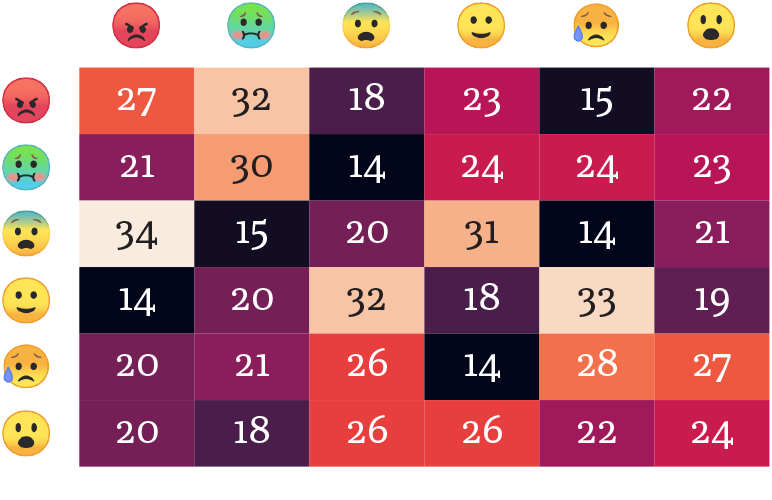
\includegraphics{imgs/confusion-emoji.png}
  \caption{Matriz de confusão do experimento de \textit{card sort}. Emoção da atriz nas linhas, classificação dos participantes nas colunas.}
  \label{matriz_confusao}
\end{marginfigure}



As entrevistas, por outro lado, trazem algumas noções que parecem iluminar melhor nossa pesquisa.

\renewcommand{\refname}{Bibliografia}
\makeatletter
\renewcommand{\bibsection}{%
   \section{\refname%
            \@mkboth{\MakeUppercase{\refname}}{\MakeUppercase{\refname}}%
   }
}
\makeatother


\bibliography{sample-handout}
\bibliographystyle{plainnat}



\end{document}